\documentclass{book}

% Packages
\usepackage{amsmath}
\usepackage[utf8]{inputenc} % Encoding
\usepackage[T1]{fontenc}  % Font encoding
\usepackage[colorlinks=true,linkcolor=blue,urlcolor=blue,citecolor=blue]{hyperref}     % Hyperlinks
\usepackage{geometry}     % Page layout
\usepackage{graphicx}
\usepackage{listings}     % Code listings
\usepackage{xcolor}       % Colors for code
\usepackage[table]{xcolor}
\usepackage{tcolorbox} % Add this to your preamble
\usepackage{tikz}
\usetikzlibrary{positioning}  

% Page layout
\geometry{margin=1in}

\tikzstyle{startstop} = [rectangle, rounded corners, minimum width=3cm, minimum height=1cm,text centered, draw=black, fill=red!30]
\tikzstyle{process} = [rectangle, minimum width=3cm, minimum height=1cm, text centered, draw=black, fill=blue!30]
\tikzstyle{file} = [rectangle, minimum width=3cm, minimum height=1cm, text centered, draw=black, fill=gray!30]
\tikzstyle{arrow} = [thick,->,>=stealth]  

% Functions
\tcbset{
    attentionbox/.style={
        colback=red!5, % Background color
        colframe=red!75!black, % Border color
        coltitle=black, % Title color
        boxrule=0.8mm, % Thickness of the border
        left=2mm, % Left padding
        before skip=5mm, % Space before the box
        after skip=5mm, % Space after the box
        sharp corners, % Sharp corners for the box
        fonttitle=\bfseries, % Bold title font
        attach boxed title to top left={yshift=-2mm,xshift=2mm}, % Title position
        boxed title style={
            size=small,
            colback=red!50,
            colframe=red!75!black,
            sharp corners,
        },
    }
}

% % Code formatting
\lstset{
    language=Python,
    basicstyle=\ttfamily\fontsize{9}{10}\selectfont,
    breaklines=true,
    frame=single,
    keywordstyle=\color{blue},
    commentstyle=\color{green!70!black},
    stringstyle=\color{red},
    showstringspaces=false,
    numbers=left,
    numberstyle=\tiny\color{gray},
    stepnumber=1,
    numbersep=10pt,
    xleftmargin=5mm,
}

\title{The HDF5\_BLS file format and its user interface}
\author{The International BioBrillouin Society}
\date{\today}

\begin{document}

\maketitle

\tableofcontents

\chapter*{Introduction}\addcontentsline{toc}{chapter}{Introduction}
    Welcome to the interactive UI tutorial. This book will guide you through the steps to create and use the UI effectively.

    The HDF5\_BLS package is a Python library for handling Brillouin light scattering (BLS) data and converting it into a standardized HDF5 format. The library provides functions to open raw data files, store their properties, convert them into a Power Spectral Density (PSD) and analyze the PSD with a standardized treatment protocol. The library is currently compatible with the following file formats:
    \begin{itemize}
        \item \textbf{*.dat} files: spectra returned by the GHOST software or obtained using Time Domain measurements
        \item \textbf{*.tif} files: an image format that can be used to export 2D detector images.
        \item \textbf{*.npy} files: an arbitrary numpy array
        \item \textbf{*.sif} files: image files obtained with Andor cameras
    \end{itemize}

    The package comes with a graphical user interface (GUI) that allows users to easily open, edit, and save data. This interface is the preferred way to use the package and the subject of this tutorial. The GUI is currently compatible with the following spectrometers:
    \begin{itemize}
        \item Tandem Fabry-Perot (TFP) spectrometers
        \item Angle-resolved VIPA (ar-VIPA) spectrometers 
    \end{itemize}

\chapter*{Preamble: The project in a nutshell}\addcontentsline{toc}{chapter}{Preamble: The project in a nutshell}

    \section*{HDF5 file structure}\addcontentsline{toc}{section}{HDF5 file structure}

        \subsection*{Basic file structure}\addcontentsline{toc}{subsection}{Basic file structure}
            The vision of the project is to unify all BLS data into a single HDF5 file. This file will be used to store all the data and metadata of the BLS. The data will be stored in a hierarchical structure, all the data related to BLS being stored the "Data" group. This choice allows results from other techinques to be stored in the same file, only in other, independent groups, to minimize the risk of nomenclature competition between techinques. The "Data" group will contain all the data. These data are arranged in groups, whose identifiers are "Data\_i". Each group can only contain one measure, in the form of an array, whose dimension is however not restricted. This measure will be called "Raw\_data". The attributes of the measure are stored in the group attributes.

            The following structure represents the base structure of the file:

            \begin{verbatim}
                file.h5
                +-- Data (group)
                |   +-- Data_1 (group)
                |   |   +-- Raw_data (dataset)
            \end{verbatim}

        \subsection*{Attributes}\addcontentsline{toc}{subsection}{Attributes}

            The attributes will follow a hierarchical structure. The attributes that apply to all "Data\_i" will be stored in the "Data" group, while the parameters that apply to a specific "Data\_i" will be stored in the "Data\_i" group. All the attributes are stored as text. Attributes are then divided in four categories:
            \begin{itemize}
                \item Attributes that are specific to the spectrometer used, such as the wavelength of the laser, the type of laser, the type of detector, etc. These attributes are recognized by the capital letter word "SPECTROMETER" in the name of the attribute.
                \item Attributes that are specific to the sample, such as the date of the measurement, the name of the sample, etc. These attributes are recognized by the capital letter word "MEASURE" in the name of the attribute.
                \item Attributes that are specific to the original file format, such as the name of the file, the date of the file, the version of the file, the precision used on the storage of the data, etc. These attributes are recognized by the capital letter word "FILEPROP" in the name of the attribute.
                \item Attributes that are used inside the HDF5 file, such as the name of the group, the name of the dataset, etc. These attributes are the only ones without a prefix.
            \end{itemize}

            The name of the attribues contains the unit of the attribute if it has units, in the shape of an underscore followed by the unit in parenthesis. Some parameters that can be represented by a series of norms will also be defined in a given norm, such as the ISO8601 for the date. These norms are however not specified in the name of the attribute. Here are some examples of attributes:
            \begin{itemize}
                \item "SPECTROMETER.Detector\_Type" is the type of the detector used.
                \item "MEASURE.Sample" is the name of the sample.
                \item "MEASURE.Exposure\_(s)" is the exposire of the sample given in seconds
                \item "MEASURE.Date\_of\_measurement" is the date of the measurement. 
                \item "FILEPROP.Name" is the name of the file.
            \end{itemize}

            To unify the name of attributes, a spreadsheet is accesible, containing all the attributes and their units. This spreadsheet will be updated as new attributes are added to the project and defined with a version number that will also be stored in the attribtutes of each data attributes (under FILEPROP.version). This spreadsheet is meant to be exported in a CSV file that can be used to update the attributes of the data.

        \subsection*{Meta-files}\addcontentsline{toc}{subsection}{Meta-files}
            It can be useful to store in a same file, measures coming from different instruments, taken in different conditions, or that we just want to separate from other groups of measures. In that end, we propose a tree-like structure of the HDF5 file, where each group can contain sub-groups, which can also contain sub-groups etc. In order to unify the way we access these groups, we propose to identify them by a unique identifier of the form "Data\_i", where "i" is an integer. Here is an example of the structure of a meta-file:

            \begin{verbatim}
                file.h5
                +-- Data
                |   +-- Data_1
                |   |   +-- Data_1
                |   |   |   +-- ...
                |   |   +-- Data_2
                |   |   |   +-- ...
                |   |   +-- ...
                |   +-- Data_2
                |   |   +-- Data_1
                |   |   |   +-- Data_1
                |   |   |   |   +-- ...
                |   |   |   +-- Data_2
                |   |   |   |   +-- ...
                |   |   |   ...
                |   |   ...
                |   ...
            \end{verbatim}

        \subsection*{Complete structure definition}\addcontentsline{toc}{subsection}{Complete structure definition}
            The file is intended to be used to store not only raw data but also treated data together with the parameters used for treatment. As such, we propose to complete the structure defined above with the following structure:

            \begin{verbatim}
                file.h5
                +-- Data (group)
                |   +-- Data_0 (group)
                |   |   +-- Raw_data (dataset)
                |   |   +-- Abscissa_0 (dataset)
                |   |   +-- Abscissa_1 (dataset)
                |   |   +-- ...
                |   |   +-- PSD (dataset)
                |   |   +-- Frequency (dataset)
                |   |   +-- Treat_0(group)
                |   |   |   +-- Shift (dataset)
                |   |   |   +-- Shift_std (dataset)
                |   |   |   +-- Linewidth (dataset)
                |   |   |   +-- Linewidth_std (dataset)
                |   |   +-- Treat_1(group)
                |   |   ...
                |   +-- Data_1 (group)
                |   ...
            \end{verbatim}

            The nomenclature is defined as follows:
            \begin{itemize}
                \item \textbf{"Data\_i"} is the identifier of the group containing the i-th measure.
                \item \textbf{"Raw\_data"} is the identifier of the dataset containing the raw data of the measure stored in the "Data\_i" group.
                \item \textbf{"Abscissa\_i"} is the identifier of the dataset containing the i-th abscissa array of "Raw\_data" and "PSD". The dimension of this dataset is not forced to one.
                \item \textbf{"PSD"} is the identifier of the dataset of the Power Spectrum Density of the measure, associated with the "Frequency" dataset. "Raw\_data" and "PSD" are arrays of same shape. We impose the last dimension(s) of "PSD" to be the same as the dimension(s) of "Frequency".
                \item \textbf{"Frequency"} is the identifier of the dataset containing the frequency axis of the "PSD".
                \item \textbf{"Treat\_i"} is the identifier of the group containing the treated data of the i-th measure.
                \item \textbf{"Shift"} is the identifier of the dataset containing the values of the fitted frequency shifts.
                \item \textbf{"Shift\_std"} is the identifier of the dataset containing the standard deviation of the fitted frequency shifts.
                \item \textbf{"Linewidth"} is the identifier of the dataset containing the values of the fitted linewidths.
                \item \textbf{"Linewidth\_std"} is the identifier of the dataset containing the standard deviation of the fitted linewidths.  
            \end{itemize}
                
    \section*{Pipeline}\addcontentsline{toc}{section}{Pipeline}

        The goal of this software is to go from a storaged data file to a usable data set with a reproducible, stable and unified treatment protocol. To schematize this treatment protocol, we propose the following diagram:

        \begin{center}
        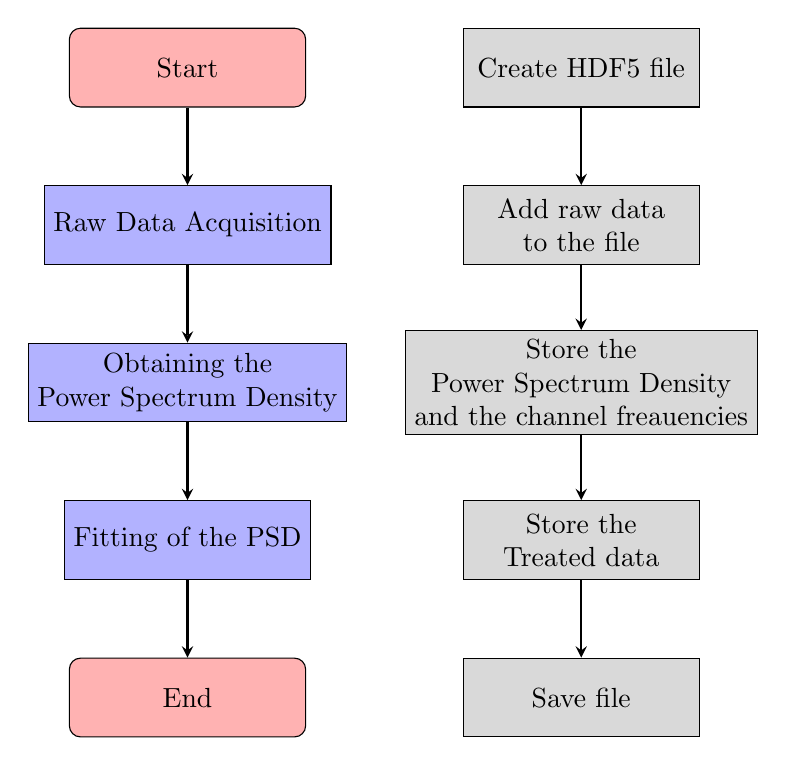
\begin{tikzpicture}[node distance=2cm]

        \node (start) [startstop] {Start};
        \node (acquire) [process, below of=start] {Raw Data Acquisition};
        \node (psd) [process, below of=acquire, align=center] {Obtaining the \\ Power Spectrum Density};
        \node (fits) [process, below of=psd] {Fitting of the PSD};
        \node (end) [startstop, below of=fits] {End};

        \draw [arrow] (start) -- (acquire);
        \draw [arrow] (acquire) -- (psd);
        \draw [arrow] (psd) -- (fits);
        \draw [arrow] (fits) -- (end);

        \node (filestart) [file, right of=start, xshift=3cm] {Create HDF5 file};
        \node (fileraw) [file, below of=filestart, align=center] {Add raw data \\ to the file};
        \node (filepsd) [file, below of=fileraw, align=center] {Store the \\ Power Spectrum Density\\and the channel freauencies};
        \node (filetreat) [file, below of=filepsd, align=center] {Store the \\ Treated data};
        \node (fileend) [file, below of=filetreat] {Save file};

        \draw [arrow] (filestart) -- (fileraw);
        \draw [arrow] (fileraw) -- (filepsd);
        \draw [arrow] (filepsd) -- (filetreat);
        \draw [arrow] (filetreat) -- (fileend);

        \end{tikzpicture}
        \end{center}

\chapter{Getting Started}
    \section{GUI quick start guide}
        To get started, you need to install the repository. Follow the instructions below:

        \begin{itemize}
            \item Step 1: Make sure you have Python 3.10 or higher installed. You can download Python at \href{https://www.python.org/downloads/}{this link}.
            \item Step 2: Clone the repository at \href{https://github.com/bio-brillouin/HDF5_BLS/tree/main}{this link}.    
            \item Step 3: Create a virtual environment and install the requirements. To do so, open a terminal, navigate to the repository folder and install the requirements. For windows users, you can open the terminal into the cloned and extracted repository (shift+left click over the folder -> Open in terminal) and use the following command:
\begin{lstlisting}
python -m venv venv
.\venv\Scripts\activate
pip install -r requirements.txt
\end{lstlisting}
            For Mac users, you can navigate to the repository, make sure you can view the path bar at the bottom of Finder (if not, check View/Show Path Bar in the menu bar), then press control and left click on the folder and select "Open in Terminal". Then, use the following command:
\begin{lstlisting}
python -m venv venv
source venv/bin/activate
pip install -r requirements.txt
\end{lstlisting}
            For Linux users, you can navigate to the repository, open a terminal in the folder and use the same command as for Mac users.
            \item Step 4: Run the \texttt{HDF5\_BLS\_GUI/main.py} file with
\begin{lstlisting}
python HDF5\_BLS\_GUI/main.py
\end{lstlisting}
        \end{itemize}

    \section{First Steps}
        \subsection{Creating a new file}
            After running all these steps, you should see the following window:

            \begin{center}
                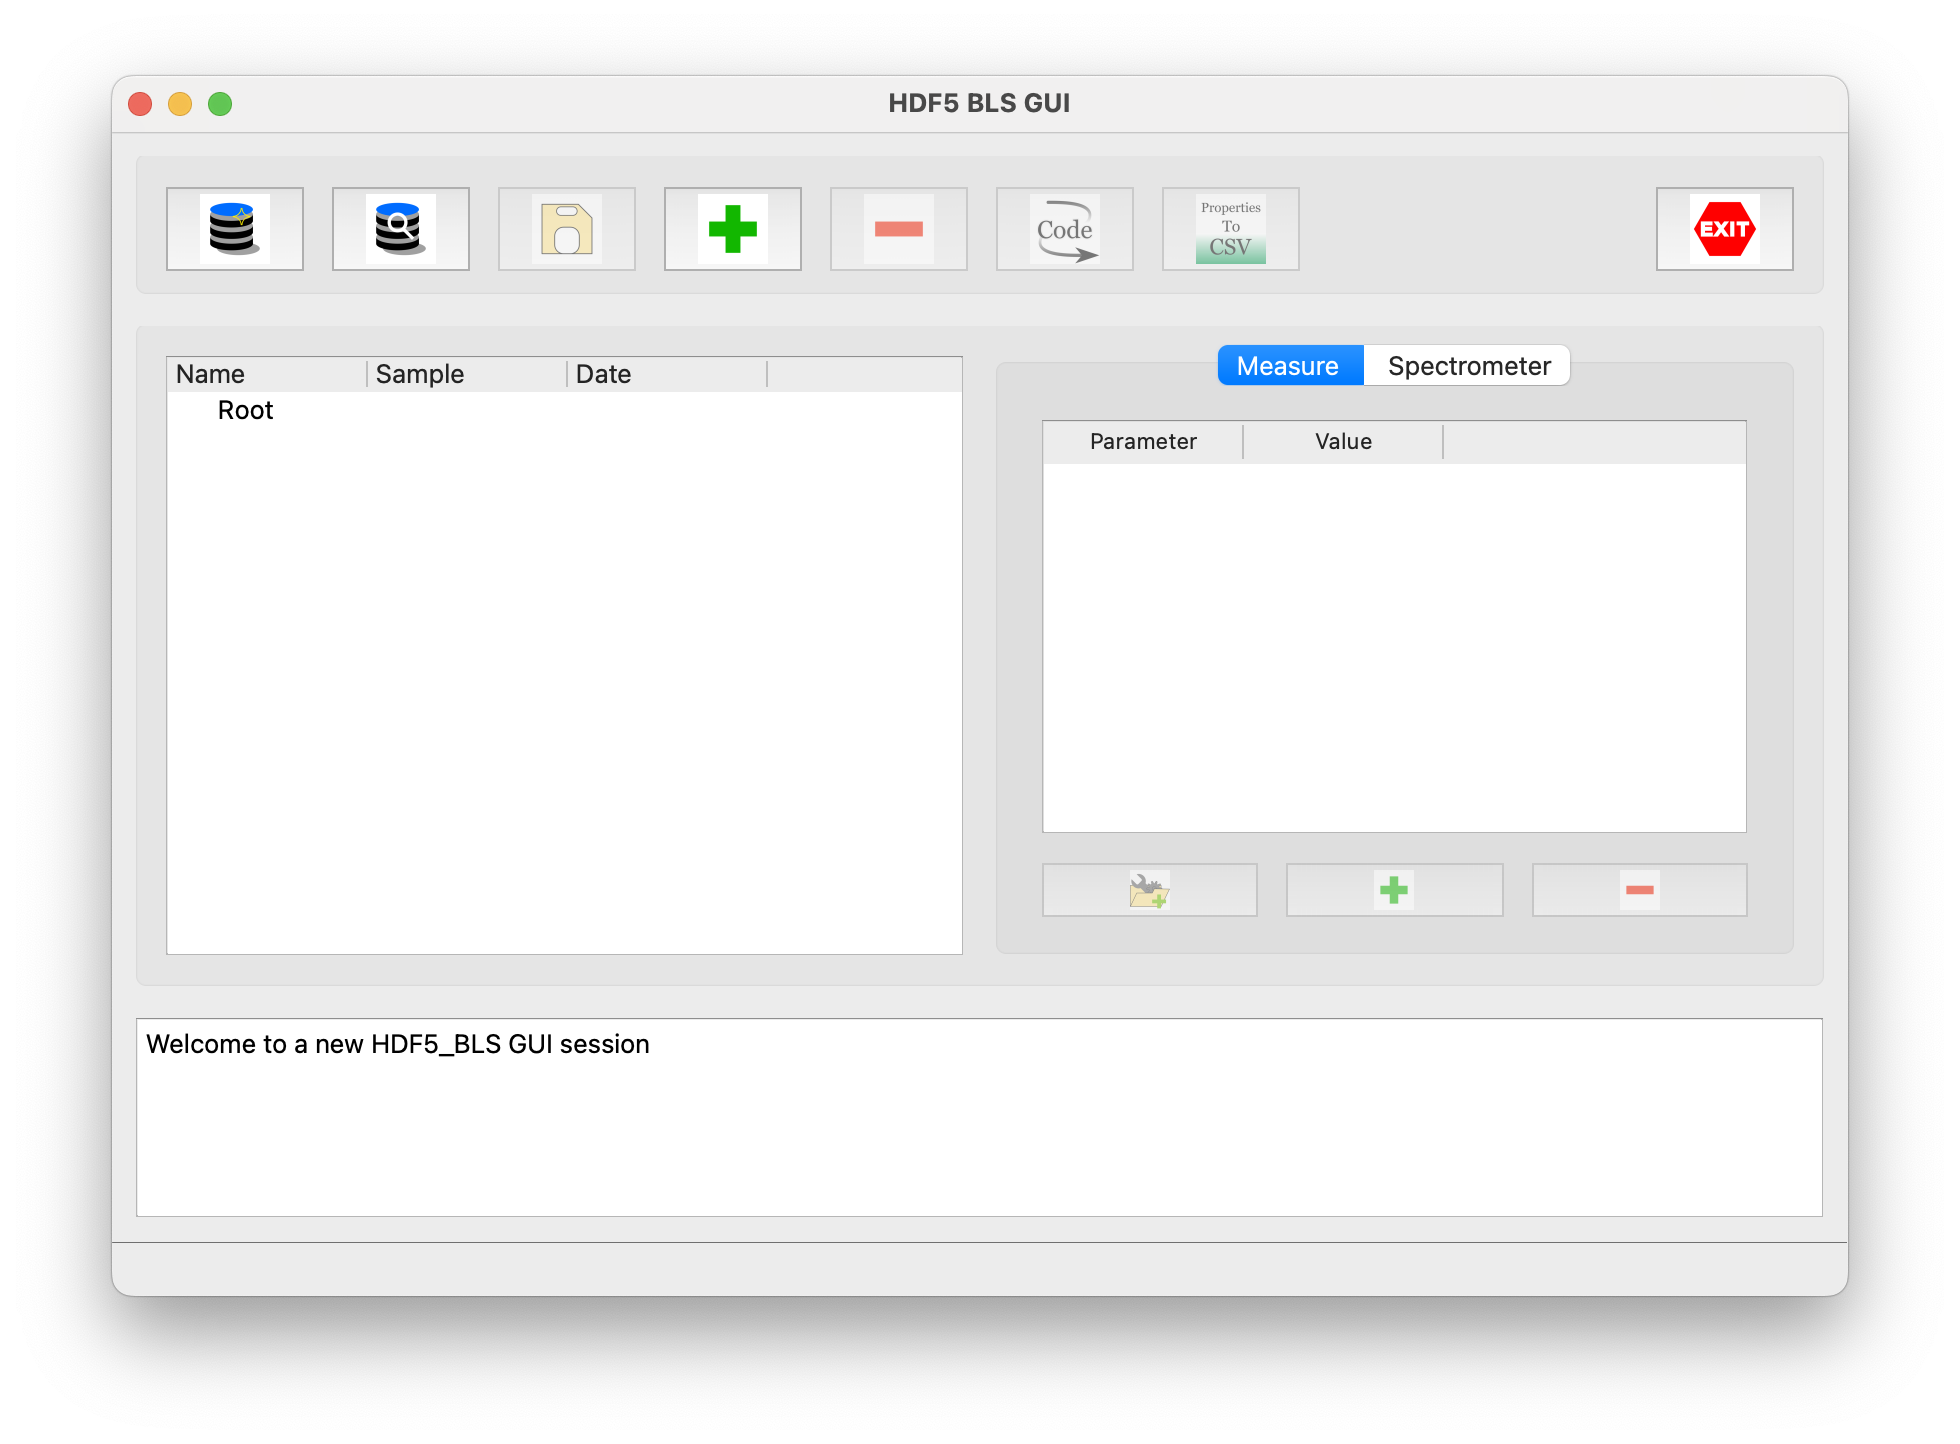
\includegraphics[width=\textwidth]{img/main_window.png}
            \end{center}

            You can then drag and drop your data into the left pannel and structure it as you wish. 
            
            You can also add properties to your data in the form of a standard CSV file which model can be found in the \texttt{spreadsheets} folder of the repository. To add a new property file to your measure, select your measure on the left pannel and drag and drop your property file to the right pannel from a file viewer. 
            
            Note that you can add property to a group of data. In that case, the property apply to all its elements.

\chapter{Development Guide} \label{chapter:dev_guide}

    \begin{tcolorbox}[title=Why are you here?]
        \begin{itemize}
            \item \hyperref[sec:load_data]{I want to import my data to the HDF5 file format}
            \item \hyperref[sec:treatment]{I want to extract information from my data }
        \end{itemize}
    \end{tcolorbox}

    \section{Load data} \label{sec:load_data}

        \begin{tcolorbox}
            Are you using a format that is already supported by the \texttt{HDF5\_BLS} package?
            \begin{itemize}
                \item \hyperref[subsec:load_data.user_specific]{Yes but it doesn't work with my data.}
                \item \hyperref[subsec:load_data.improvement]{Yes but I would like to improve the code.}
                \item \hyperref[subsec:load_data.new_format]{No, I would like to add support for my data.}
            \end{itemize}
        \end{tcolorbox}

        \subsection{Adding a user-specific function to an already supported format} \label{subsec:load_data.user_specific}

            \begin{tcolorbox}
                You are in the situation where you are using a format that is already supported by the \texttt{HDF5\_BLS} package (for example ".dat") but that doesn't work with your data.
            \end{tcolorbox}

            Here are the steps to follow:
            \begin{enumerate}
                \item Locate the python file that handles your data format in the \texttt{load\_formats} folder of the \texttt{HDF5\_BLS} package. The name of the file should correspond to the name of the format you are using (for example "load\_dat.py" if you are using ".dat" files).
                \item Add the function that will load your data to the file. The function should have the following signature:
\begin{lstlisting}
def load_dat_Wien(filepath, parameters = None):
\end{lstlisting}
                In the case where you don't need to load the data with parameters, the function should have the following signature:
\begin{lstlisting}
def load_dat_Wien(filepath):
\end{lstlisting}
                \item Write the code that will load your data. Your function should retunr a dictionnary with at least two keys: "Data" and "Attributes". The "Data" key should contain the data you are loading and the "Attributes" key should contain the attributes of the file. You can also add abscissa to your data if you want to, in that case, add the key "Abscissa\_\textsl{name}" where \textsl{name} is the name you want to give to the abscissa (for example "Abscissa\_Time").
                \item Go to the \texttt{load\_data.py} file in the \texttt{HDF5\_BLS} package and locate the function dedicated to the format you are using (for example "load\_dat\_file" if you are using ".dat" files)
                \item Make sure that you are importing the function you just created:
\begin{lstlisting}
from HDF5_BLS.load_formats.load_dat import load_dat_Wien
\end{lstlisting}
                \item Then, define an identifier for your function (for example "Wien") and either create or add your identifier to the if-else statement. Don't forget to add your identifier to the "creator\_list" list in the "else" statement:
\begin{lstlisting}
if creator == "GHOST": return load_dat_GHOST(filepath)
...
elif creator == "Wien": return load_dat_Wien(filepath)
else:
    creator_list = ["GHOST", "TimeDomain", "Wien"]
    raise LoadError_creator(f"Unsupported creator {creator}, accepted values are: {', '.join(creator_list)}", creator_list)
\end{lstlisting}
                \item Add a test to the function in the "tests/load\_data\_test.py" file with a test file placed in the "tests/test\_data" folder. This test is important as they are run automatically when the package is pushed to GitHub (ie: it makes my life easier ^^). 
                \item You can now use your data format with the \texttt{HDF5\_BLS} package, and in particular, the GUI. You are invited to push your code to GitHub and create a pull request to the main repository :)
            \end{enumerate}

        \subsection{Improving an already supported function} \label{subsec:load_data.improvement}
            \begin{tcolorbox}
                You are in the situation where you want to improve a load function of the \texttt{HDF5\_BLS} package (for example ".dat").
            \end{tcolorbox}

            Here are the steps to follow:
            \begin{enumerate}
                \item Locate the python file that handles your data format in the \texttt{load\_formats} folder of the \texttt{HDF5\_BLS} package. The name of the file should correspond to the name of the format you are using (for example "load\_dat.py" if you are using ".dat" files).
                \item Locate the function that loads your data. The function should have a name similar to (might not have parameters):
\begin{lstlisting}
def load_dat_Wien(filepath, parameters = None):
\end{lstlisting}
                \item Update the code. One good measure is to duplicate the function and comment one of the two versions. Then, write your code and run the tests. If the tests fail, you can always go back to the previous version. Note that if the test fails, the code cannot be pushed to GitHub.
                \item If everything is sound, you can now use your new function with the \texttt{HDF5\_BLS} package. You are invited to push your code to GitHub and create a pull request to the main repository :)
                \item Note: If you want to improve the loading of the data to the hdf5 file (chunking for example), please contact the maintainer directly.
        \end{enumerate}

        \subsection{Adding a user-specific function to an already supported format} \label{subsec:load_data.new_format}

            \begin{tcolorbox}
                You are in the situation where you are using a new format that is not supported by the \texttt{HDF5\_BLS} package.
            \end{tcolorbox}

            Here are the steps to follow:
            \begin{enumerate}
                \item Navigate to the \texttt{load\_formats} folder of the \texttt{HDF5\_BLS} package. 
                \item Create a new python file with the name of the format you are using (for example "load\_unicorn.py" if you are using ".unicorn" files).
                \item Add the function that will load your data to the file. The function should have the following signature:
\begin{lstlisting}
def load_unicorn_Wien(filepath, parameters = None):
\end{lstlisting}
                In the case where you don't need to load the data with parameters, the function should have the following signature:
\begin{lstlisting}
def load_dat_Wien(filepath):
\end{lstlisting}
                \item Write the code that will load your data. Your function should retunr a dictionnary with at least two keys: "Data" and "Attributes". The "Data" key should contain the data you are loading and the "Attributes" key should contain the attributes of the file. You can also add abscissa to your data if you want to, in that case, add the key "Abscissa\_\textsl{name}" where \textsl{name} is the name you want to give to the abscissa (for example "Abscissa\_Time").
                \item Go to the \texttt{load\_data.py} file in the \texttt{HDF5\_BLS} package and create the function dedicated to the format you are using (for example "load\_unicorn\_file" if you are using ".unicorn" files)
                \item Make sure that you are importing the function you just created:
\begin{lstlisting}
from HDF5_BLS.load_formats.load_unicorn import load_unicorn_Wien
\end{lstlisting}
                \item Add a test to the function in the "tests/load\_data\_test.py" file with a test file placed in the "tests/test\_data" folder. This test is important as they are run automatically when the package is pushed to GitHub (ie: it makes my life easier ^^). 
                \item You can now use your data format with the \texttt{HDF5\_BLS} package, and in particular, the GUI. You are invited to push your code to GitHub and create a pull request to the main repository :)
            \end{enumerate}

    \section{Treat data} \label{sec:treatment}

        \begin{tcolorbox}
            What is the format of your data?
            \begin{itemize}
                \item \hyperref[subsec:treatment.toPSD]{I just have raw data coming from the spectrometer}
                \item \hyperref[subsec:treatment.toInfo]{I have a Spectral Power Density together with a frequnecy vector}
                \item \hyperref[subsec:treatment.new]{I want to define a new treatment function}
            \end{itemize}
        \end{tcolorbox}

        \subsection{Treat data to obtain a Power Spectral Density and a frequency vector} \label{subsec:treatment.toPSD}
            \begin{tcolorbox}
                To do
            \end{tcolorbox}

        \subsection{Treat data to extract information from a Power Spectral Density} \label{subsec:treatment.toInfo}

            Here are the steps to follow for the GUI compatibility:
            \begin{enumerate}
                \item If "type" is the type of your spectrometer, add the function "treat\_type" in the "HDF5\_BLS\_GUI/treat\_ui.py" file. For example if your spectrometer type is "Unicorn", add the following function:
\begin{lstlisting}
def treat_unicorn
\end{lstlisting}
                \item Add the following parameters to your function:
                \begin{itemize}
                    \item parent: the parent GUI window
                    \item wrp: the wrapper associated to the main h5 file
                    \item path: the path to the data we want to treat in the form "Data/Data/..."
                \end{itemize}
\begin{lstlisting}
def treat_unicorn(parent, wrp, path):
\end{lstlisting}
                \item Define your function. You can find an example of how it was done for the "TFP" treatment in the \hyperref[subsec:example_treatment.TFP]{appendix}.
            \end{enumerate}
        
        \subsection{Adding a new treatment function} \label{subsec:treatment.new}

\chapter*{Contact}\addcontentsline{toc}{chapter}{Contacts}
    For questions or suggestions, please contact the maintainer at:

    \begin{center}
        \href{mailto:pierre.bouvet@meduniwien.ac.at}{pierre.bouvet@meduniwien.ac.at}.
    \end{center}




\appendix

\part*{Appendix}\addcontentsline{toc}{part}{Appendix}

\chapter{Examples of file structures}
        
    \section{A single measure with no treatment}
        In this first example, we want to store a single measure of a water sample.
    
        The following structure represents the base structure of the file:
        \begin{verbatim}
            file.h5
            +-- Data (group) -> Name = "Measure"
            |   +-- Data_0 (group) -> Name = "Water"
            |   |   +-- Raw_data (dataset)
        \end{verbatim}
        Note that we have here added arrows and an example of the value of the "Name" attributes.
    
    \section{A series of measures with no treatment}
        In this second example, we want to store a series of measures taken on three different samples: Water, Ethanol and Glycerol.

        The following structure represents the base structure of the file:
        \begin{verbatim}
            file.h5
            +-- Data (group) -> Name = "Measure"
            |   +-- Data_0 (group) -> Name = "Water"
            |   |   +-- Raw_data (dataset)
            |   +-- Data_1 (group) -> Name = "Ethanol"
            |   |   +-- Raw_data (dataset)
            |   +-- Data_2 (group) -> Name = "Glycerol"
            |   |   +-- Raw_data (dataset)
        \end{verbatim}
        Note that we have here added arrows and an example of the value of the "Name" attributes.
    
    \section{A series of series of measures with no treatment but with a calibration spectrum and an impulse response measure}
        In this third example, we want to store a series of two measures taken on two different samples: Water and Ethanol. We also want to store a calibration curve and an impulse response curve.

        The following structure represents the base structure of the file:
        \begin{verbatim}
            file.h5
            +-- Data (group) -> Name = "Measure"
            |   +-- Data_0 (group) -> Name = "Impulse_Response"
            |   |   +-- Raw_data (dataset)
            |   +-- Data_1 (group) -> Name = "Calibration"
            |   |   +-- Raw_data (dataset)
            |   +-- Data_2 (group) -> Name = "Water"
            |   |   +-- Data_0 (group) -> Name = "Water_01"
            |   |   |   +-- Raw_data (dataset)
            |   |   +-- Data_1 (group) -> Name = "Water_02"
            |   |   |   +-- Raw_data (dataset)
            |   +-- Data_3 (group) -> Name = "Ethanol"
            |   |   +-- Data_0 (group) -> Name = "Ethanol_01"
            |   |   |   +-- Raw_data (dataset)
            |   |   +-- Data_1 (group) -> Name = "Ethanol_02"
            |   |   |   +-- Raw_data (dataset)
        \end{verbatim}
        Note that we have here added arrows and an example of the value of the "Name" attributes.
    
    \section{A single measure converted to a Power Spectrum Density}
        In this fourth example, we want to store a single measure of a water sample. This measure has been converted into a Power Spectrum Density.

        The following structure represents the base structure of the file:
        \begin{verbatim}
            file.h5
            +-- Data (group) -> Name = "Measure"
            |   +-- Data_0 (group) -> Name = "Water"
            |   |   +-- Raw_data (dataset)
            |   |   +-- PSD (dataset)
            |   |   +-- Frequency (dataset)
        \end{verbatim}
        Note that we have here added arrows and an example of the value of the "Name" attributes.
        In this case, all the steps of the conversion to PSD are stored in the "Data\_0" group. The nomenclature of the attribute(s) used to store the parameters of the treatment is not specified.
    
    \section{Multiple measures converted to a Power Spectrum Density with a time-independent spectrometer}
        In this fifth example, we are in the situation where a time-independent spectrometer has been used to acquire multiple measures. In this case, the hierrarchy of the file can be used to reduce the number of datasets, by considering that all the PSD share the same frequency axis.

        The following structure represents the base structure of the file:
        \begin{verbatim}
            file.h5
            +-- Data (group) -> Name = "Measure"
            |   +-- Frequency (dataset)
            |   +-- Data_0 (group) -> Name = "Sample_1"
            |   |   +-- Raw_data (dataset)
            |   |   +-- PSD (dataset)
            |   +-- Data_1 (group) -> Name = "Sample_2"
            |   |   +-- Raw_data (dataset)
            |   |   +-- PSD (dataset)
        \end{verbatim}
        Note that we have here added arrows and an example of the value of the "Name" attributes.

    \section{A single measure with a treatment}
        In this sixth example, we want to store a single measure of a water sample that has been treated.

        The following structure represents the base structure of the file:
        \begin{verbatim}
            file.h5
            +-- Data (group) -> Name = "Measure"
            |   +-- Data_0 (group) -> Name = "Water"
            |   |   +-- Raw_data (dataset)
            |   |   +-- PSD (dataset)
            |   |   +-- Frequency (dataset)
            |   |   +-- Treat_0 (group) -> Name = "Treat_5GHz"
            |   |   |   +-- Shift (dataset)
            |   |   |   +-- Shift_std (dataset)
            |   |   |   +-- Linewidth (dataset)
            |   |   |   +-- Linewidth_std (dataset)
        \end{verbatim}
        Note that we have here added arrows and an example of the value of the "Name" attributes.
        In this case, all the steps of the treatment are stored in the "Treat\_0" group. The nomenclature of the attribute(s) used to store the parameters of the treatment is not specified.
    
    \section{A single measure with two distinct treatments}
        In this seventh example, we will store a single measure where two different treatments have been performed (for example a measure at an interface between two materials).

        The following structure represents the base structure of the file:
        \begin{verbatim}
            file.h5
            +-- Data (group) -> Name = "Measure"
            |   +-- Data_0 (group) -> Name = "Water"
            |   |   +-- Raw_data (dataset)
            |   |   +-- PSD (dataset)
            |   |   +-- Frequency (dataset)
            |   |   +-- Treat_0 (group) -> Name = "Treat_5GHz"
            |   |   |   +-- Shift (dataset)
            |   |   |   +-- Shift_std (dataset)
            |   |   |   +-- Linewidth (dataset)
            |   |   |   +-- Linewidth_std (dataset)
            |   |   +-- Treat_1 (group) -> Name = "Treat_10GHz"
            |   |   |   +-- Shift (dataset)
            |   |   |   +-- Shift_std (dataset)
            |   |   |   +-- Linewidth (dataset)
            |   |   |   +-- Linewidth_std (dataset)
        \end{verbatim}
        Note that we have here added arrows and an example of the value of the "Name" attributes.
        In this case, all the steps of the treatment around 5GHz are stored in the "Treat\_0" group and the ones around 10GHz in the "Treat\_1" group. The nomenclature of the attribute(s) used to store the parameters of the treatment is not specified.

    \section{A single mapping stored as a single measure}
        In this eighth example, we want to store a mapping of a sample. This mapping has been obtained with a spectrometer that returns an array of points for all the points mapped. To clarify this example, we will indicate the dimension of each dataset here between brackets.

        The following structure represents the base structure of the file:
        \begin{verbatim}
            file.h5
            +-- Data (group) -> Name = "Measure"
            |   +-- Data_0 (group) -> Name = "Sample"
            |   |   +-- Raw_data (dataset) [X, Y, M]
            |   |   +-- PSD (dataset) [X, Y, N]
            |   |   +-- Frequency (dataset) [N]
            |   |   +-- Abscissa_0 (dataset) [X] -> Name = "x (mm)"
            |   |   +-- Abscissa_1 (dataset) [Y] -> Name = "y (mm)"
            |   |   +-- Treat_1 (group) -> Name = "Treat"
            |   |   |   +-- Shift (dataset) [X, Y]
            |   |   |   +-- Shift_std (dataset) [X, Y]
            |   |   |   +-- Linewidth (dataset) [X, Y]
            |   |   |   +-- Linewidth_std (dataset) [X, Y]
        \end{verbatim}
        Note that we have here added arrows and an example of the value of the "Name" attributes.
    
    \section{A series of mapping over the same field of view stored as a single measure}
        In this ninth example, we are in the situation where multiple mappings of same dimension have been obtained with a spectrometer that returns an array of points for all the points mapped. In this case, the hierrarchy of the file can be used to reduce the number of datasets, by considering that all the PSD share the same frequency axis and the same field of view.

        The following structure represents the base structure of the file:
        \begin{verbatim}
            file.h5
            +-- Data (group) -> Name = "Measure"
            |   +-- Abscissa_0 (dataset) [X] -> Name = "x (mm)"
            |   +-- Abscissa_1 (dataset) [Y] -> Name = "y (mm)"
            |   +-- Frequency (dataset) [N]
            |   +-- Data_0 (group) -> Name = "Day_1"
            |   |   +-- Raw_data (dataset) [X, Y, M]
            |   |   +-- PSD (dataset) [X, Y, N]
            |   |   +-- Treat_1 (group) -> Name = "Treat"
            |   |   |   +-- Shift (dataset) [X, Y]
            |   |   |   +-- Shift_std (dataset) [X, Y]
            |   |   |   +-- Linewidth (dataset) [X, Y]
            |   |   |   +-- Linewidth_std (dataset) [X, Y]
            |   +-- Data_1 (group) -> Name = "Day_2"
            |   |   +-- Raw_data (dataset) [X, Y, M]
            |   |   +-- PSD (dataset) [X, Y, N]
            |   |   +-- Treat_1 (group) -> Name = "Treat"
            |   |   |   +-- Shift (dataset) [X, Y]
            |   |   |   +-- Shift_std (dataset) [X, Y]
            |   |   |   +-- Linewidth (dataset) [X, Y]
            |   |   |   +-- Linewidth_std (dataset) [X, Y]
        \end{verbatim}
        Note that we have here added arrows and an example of the value of the "Name" attributes.
    
    \section{A series of mapping over the same field of view stored as multiple measures}
        In this tenth example, we are in the situation where multiple mappings of same dimension have been obtained with a spectrometer that can't return an array of points for all the points mapped, but returns them one by one. Because it would be impractical to create groups for each point, we encourage users to compile their data into a single dataset, and refer to example 9.
    
    \section{A series of mapping obtained with different spectrometers and with different field of view}
        In this eleventh example, we are in the situation where multiple mappings of different dimensions have been obtained with different spectrometers that all return an array of points for all the points mapped. In this case, the hierrarchy of the file cannot be used to reduce the number of datasets, and each group will need its own abscissa and frequency datasets.

            The following structure represents the base structure of the file:
            \begin{verbatim}
                file.h5
                +-- Data (group) -> Name = "Measure"
                |   +-- Data_0 (group) -> Name = "VIPA"
                |   |   +-- Raw_data (dataset) [X, Y, M]
                |   |   +-- PSD (dataset) [X, Y, N]
                |   |   +-- Abscissa_0 (dataset) [X] -> Name = "x (mm)"
                |   |   +-- Abscissa_1 (dataset) [Y] -> Name = "y (mm)"
                |   |   +-- Frequency (dataset) [N]
                |   |   +-- Treat_1 (group) -> Name = "Treat"
                |   |   |   +-- Shift (dataset) [X, Y]
                |   |   |   +-- Shift_std (dataset) [X, Y]
                |   |   |   +-- Linewidth (dataset) [X, Y]
                |   |   |   +-- Linewidth_std (dataset) [X, Y]
                |   +-- Data_1 (group) -> Name = "TFP"
                |   |   +-- Raw_data (dataset) [X, Y, M]
                |   |   +-- PSD (dataset) [X, Y, N]
                |   |   +-- Abscissa_0 (dataset) [X] -> Name = "x (mm)"
                |   |   +-- Abscissa_1 (dataset) [Y] -> Name = "y (mm)"
                |   |   +-- Frequency (dataset) [N]
                |   |   +-- Treat_1 (group) -> Name = "Treat"
                |   |   |   +-- Shift (dataset) [X, Y]
                |   |   |   +-- Shift_std (dataset) [X, Y]
                |   |   |   +-- Linewidth (dataset) [X, Y]
                |   |   |   +-- Linewidth_std (dataset) [X, Y]
            \end{verbatim}
            Note that we have here added arrows and an example of the value of the "Name" attributes.

\chapter{Examples of treatment pipelines}

    \section{Treatment of a TFP spectrometer} \label{subsec:example_treatment.TFP}

        \begin{tcolorbox}
            We here present the code that was used to treat the data obtained from a TFP spectrometer. This code is meant to be used as an example of how to write a treatment function for the GUI compatibility. 
        \end{tcolorbox}

        \begin{enumerate}
            \item We first extract all the PSDs and frequency arrays that are child of the element that has been selected. To do that, we need to go through all the higher layers of our wrapper until our data is found. This is done using the following code:
\begin{lstlisting}
def get_paths_childs(wrp, path = "", frequency = None):
    child, freq = [], []
    if "Frequency" in wrp.data.keys():
        frequency = path+"/Frequency"
    for e in wrp.data.keys():
        if isinstance(wrp.data[e], wrapper.Wrapper):
            ce, fe = get_paths_childs(wrp.data[e], path+"/"+e, frequency=frequency)
            child += ce
            freq += fe
        else:
            if e == "Power Spectral Density":
                freq.append(frequency)
                child.append(path+"/"+e)
    return child, freq
        
# Get the selected data wrapper and frequency array
wrp_temp = wrp
path_loc = path.split("/")[1:]
if "Frequency" in wrp.data.keys(): frequency = wrp.data["Frequency"]
else: frequency = None
for e in path_loc: 
    if "Frequency" in wrp_temp.data[e].data.keys(): 
        frequency = wrp_temp.data[e].data["Frequency"]
    if isinstance(wrp_temp.data[e], wrapper.Wrapper): 
        wrp_temp = wrp_temp.data[e]

childs, frequency = get_paths_childs(wrp_temp, path)
\end{lstlisting}
        \item From there we have a choice to make: either we treat each PSD individually or all at once, from some globally defined parameters. We therefore need to ask the user if he wants to treat all of them with the same parameters or each one individually. This is done using the following code:
\begin{lstlisting}
# Display a dialog box to ask the user if he wants to treat all of them with the same parameters or each one individually
msgBox = qtw.QMessageBox()        
msgBox.setText(f"There are {len(childs)} PSD in the selected data. Do you want to treat all of them at once?")
msgBox.setStandardButtons(qtw.QMessageBox.Yes | qtw.QMessageBox.No | qtw.QMessageBox.Cancel)
msgBox.setDefaultButton(qtw.QMessageBox.Yes)
ret = msgBox.exec()
if ret == qtw.QMessageBox.Yes: 
    # Treat all PSD at once
elif ret == qtw.QMessageBox.No:
    # Treat each PSD individually
\end{lstlisting}
        \item In both cases, we will want to open a window to enter the parameters of the treatment. In the first case, where all the spectra are treated at once, we open the window with all the spectra as parameters. In the second case, where each spectrum is treated individually, we will have a "for" loop to open the window for each spectrum. This is done using the following code:
\begin{lstlisting}
from ParameterCurve.main import TFP_treat

if ret == qtw.QMessageBox.Yes: 
    dialog = TFP_treat(parent = parent, wrp_base = wrp, path_base = path, path_curves = childs, path_frequency = frequency)
    if dialog.exec_() == qtw.QDialog.Accepted:
        # Store all the treated values
elif ret == qtw.QMessageBox.No:
    for c,f in zip(childs, frequency):
        dialog = TFP_treat(parent = parent, wrp_base = wrp, path_base = path, path_curves = childs, path_frequency = frequency)
        if dialog.exec_() == qtw.QDialog.Accepted:
            # Store the treated values
\end{lstlisting}
        Note that here we are importing another GUI window from the \texttt{ParameterCurve} package. The definition of this GUI window is therefore the next step. Let's now look into this \texttt{TFP\_treat} class.
        \item Opening the "HDF5\_BLS\_GUI/ParameterCurve/main.py" file, we define the \texttt{TFP\_treat} class as a daughter of the \texttt{ParameterCurve} class, which is a GUI window with 4 distinct elements:
        \begin{itemize}
            \item A combobox to select the curves to plot at the top left of the window.
            \item A combobox to select the function to apply at the top right of the window.
            \item A graph frame to display the curves at the bottom left of the window.
            \item A frame to display the parameters of the treatment at the bottom right of the window, together with buttons to apply the treatment and to close the window.
        \end{itemize}:
\begin{lstlisting}
class TFP_treat(ParameterCurve):
    def __init__(self, parent=None, wrp_base = None, path_base = None, path_curves = None, path_frequency = None):
        super().__init__(parent, wrp_base.get_child(path_base))
\end{lstlisting}
        This initializes the \texttt{ParameterCurve} class with the wrapper corresponding to all the curves we are going to treat. Giving the class the path of the selected curves displays them by default in the combobox.
        Here is an image of a raw ParameterCurve window after this simple initialization:
        \begin{center}
            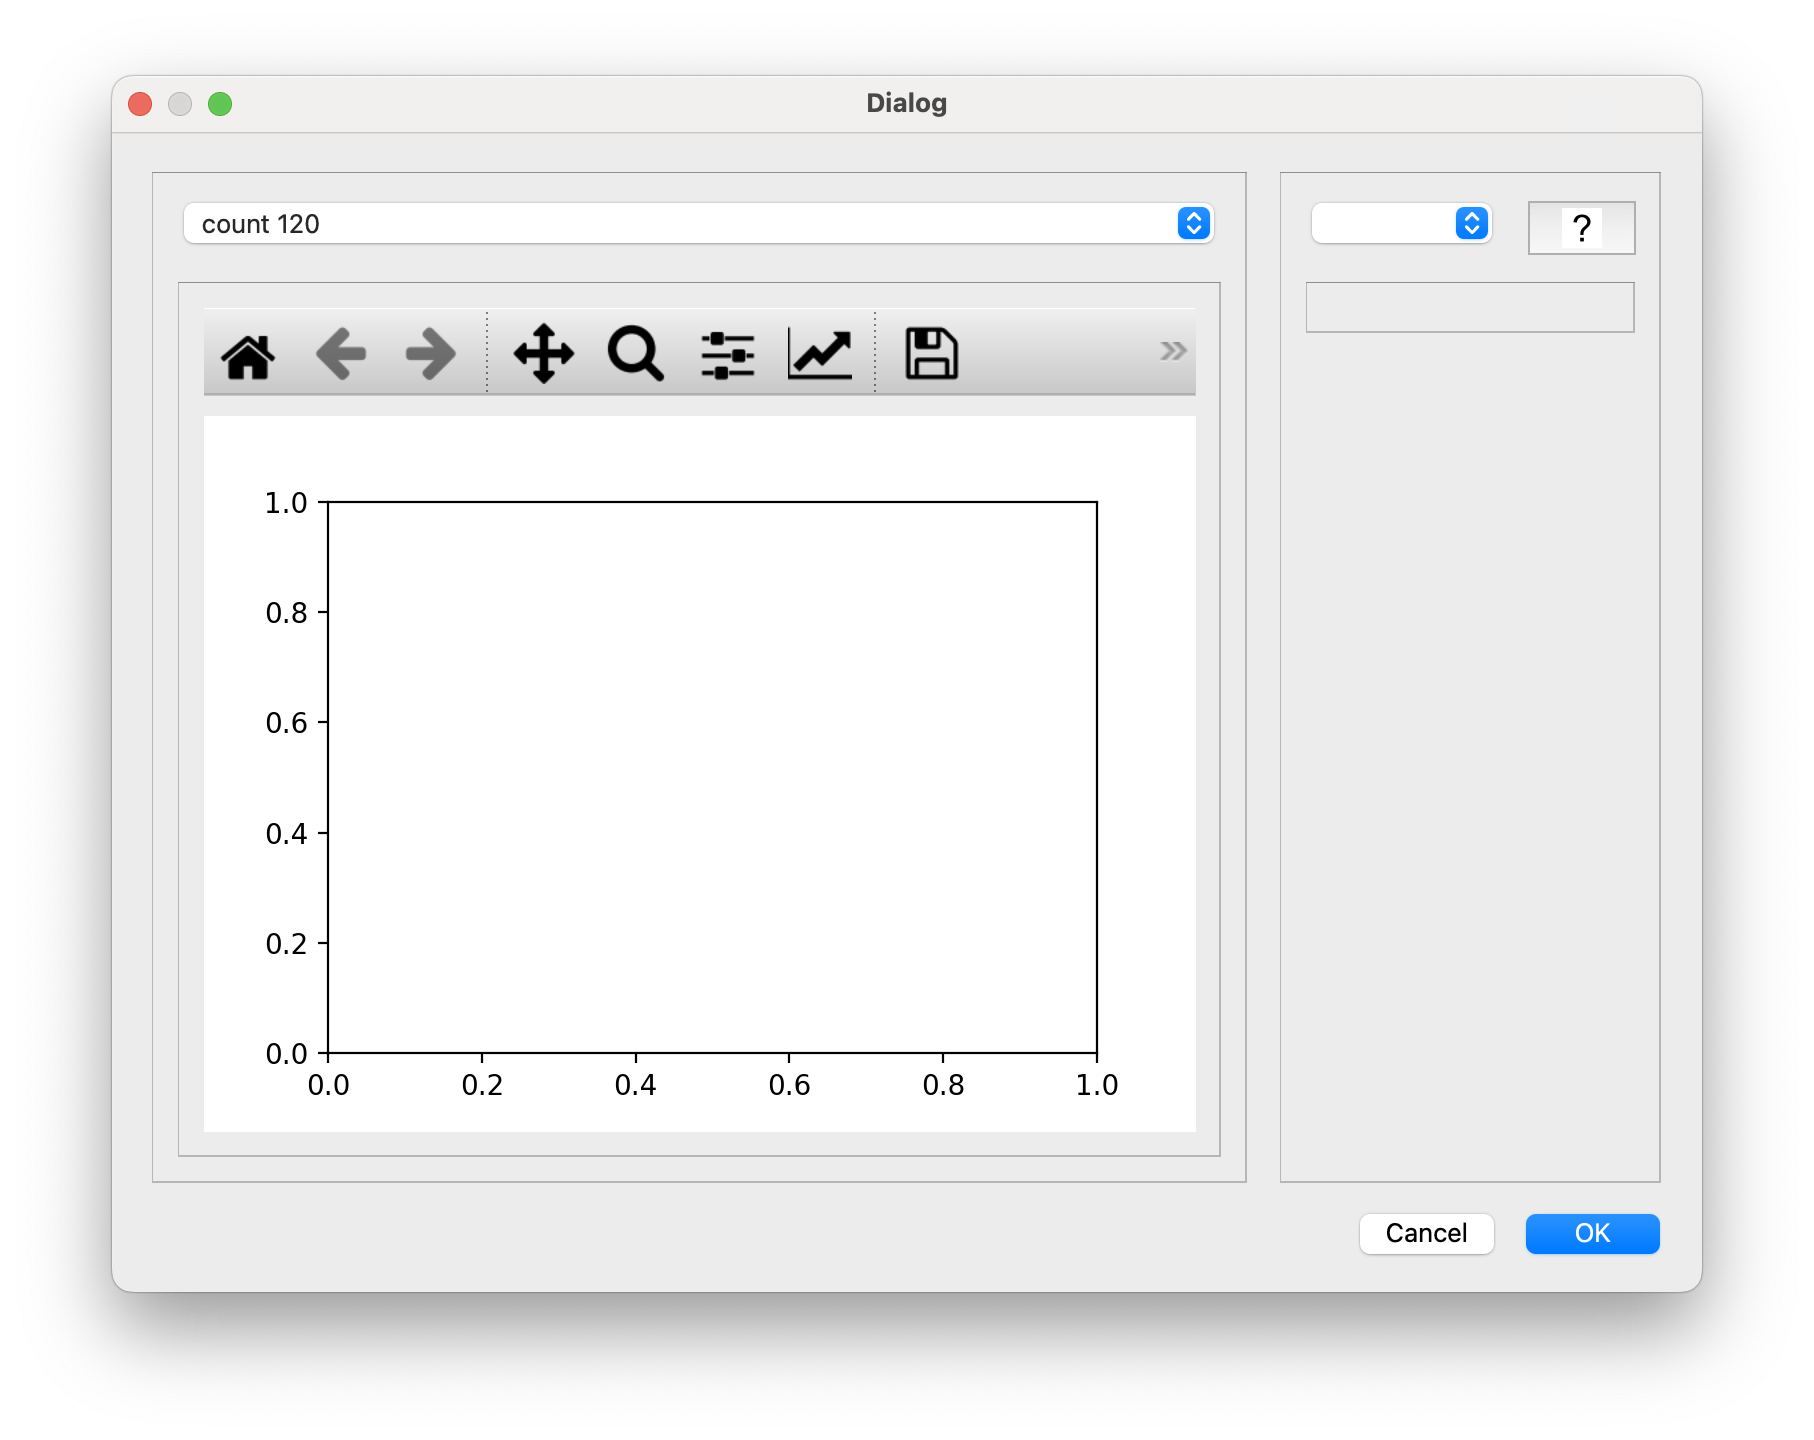
\includegraphics[width=\textwidth]{img/ParameterCurve.png}
        \end{center}
        \item We can now add functionailities to the GUI. First, we display the curve that we select in the combobobx. To do so, we will call the \texttt{handle\_data} function when the combobox is changed. This function will extract the data from the wrapper corresponding to the selected curve and plot it on the graph.
\begin{lstlisting}
def __init__(self, parent=None, wrp_base = None, path_base = None, path_curves = None, path_frequency = None, frequency = None):
    super().__init__(parent, wrp_base.get_child(path_base))

    if frequency is None:
        self.path_curves = path_curves
        self.path_frequency = path_frequency
        self.path_frequency_unique = None
    else:
        self.path_curves = None
        self.path_frequency = None
        self.path_frequency_unique = frequency

    # Initializes the graph
    self.cb_curves.currentIndexChanged.connect(self.handle_data)
\end{lstlisting}
        Note that we have also stored the paths to the frequencies associated to the curves in respectively the \texttt{path\_frequency} and \texttt{path\_curves} attributes. In the case where only one array is shown, then the path to the frequency array is stored in the \texttt{path\_frequency\_unique} attribute. 
        \item The \texttt{handle\_data} function extracts the path associated to a value in the combobox and gets both the Power Spectral Density and the frequency array from the wrapper corresponding to the selected curve. It then plots the data on the graph.
\begin{lstlisting}
def handle_data(self):
    """
    Plots the curve that is currently selected in the combobox. This function also defines self.data and updates the parameters.
    """
    # Extract the raw data from the wrapper corresponding to the selected curve in the combobox
    wrp = self.wrapper
    
    if len(self.combobox_curve_codes) > 1:
        path = self.combobox_curve_codes[self.combobox_curve_names.index(self.cb_curves.currentText())]
        path = path[5:]

        if type(path) == list:
            for e in path:
                wrp = wrp.data[e]
        else:
            wrp = wrp.data[path]
        
        self.data = wrp.data["Power Spectral Density"]
        if self.path_frequency is None:
            self.frequency = wrp.get_child(self.path_frequency_unique)[:]
        else:
            self.frequency = wrp.get_child(self.path_frequency[self.path_curves.index(path+"/Power Spectral Density")])[:]
        
        # Plot the data
        self.graph_canvas.axes.cla()

        self.graph_canvas.axes.plot(self.frequency, self.data)
        self.graph_canvas.axes.set_xlabel("Frequency Shift (GHz)")
        self.graph_canvas.axes.set_ylabel("Intensity (AU)")
        self.graph_canvas.draw()
        self.update_parameters()
\end{lstlisting}
        Note that the last line of this function is calling the function \texttt{update\_parameters}. This function will update the list of parameters needed to run the treatment. 
        \item We can define the \texttt{update\_parameters} function. This function will most likely be common to most treatments. Its goal is to inspect the "treat" module from the \texttt{HDF5\_BLS} package and extract the list of functions and parameters that are needed automatically. Then it displays the list of functions in the dedicated combobox and the list of parameters in the dedicated frame. If the nomenclature of the parameters and the definition of the treatment function follow a fixed nomenclature, this function automatically links the graph with the relevant parameters so that the graph becomes interactive. Further information about how to develop new treatment functions can be found in section \hyperref[subsec:treatment.new]{Adding a new treatment function}. Out of curiosity, here is the detail of the code of this function:
\begin{lstlisting}
def update_parameters(self):
    def initialize_parameters(self, module):
        functions = [func for func in getmembers(module, isfunction)]
        function_names = [func[0] for func in functions]
        functions = [func[1] for func in functions]

        self.cb_functions.clear()
        self.cb_functions.addItems(function_names)
        self.cb_functions.setCurrentIndex(0)
        self.cb_functions.currentIndexChanged.connect(lambda: self.show_parameters_function(functions, function_names))

        return functions, function_names

    def setup_button_help_function(self, functions, function_names):
        def show_help_function():
            docstring = functions[function_names.index(self.function_name)].__doc__ or ""
            msgBox = HelpFunction(self, self.function_name, docstring)
            msgBox.exec_()

        self.b_helpFunction.clicked.connect(show_help_function)

    def onclick_x0(event = None):
        if event.inaxes:
            x = float(event.xdata) * 1e6//1
            x = x/1e6
            self.parameters["center_frequency"]["line_edit"].setText(str(x))
    
    def onclick_linewidth(event = None):
        if event.inaxes:
            self.temp_linewidth = float(event.xdata)
            self.graph_canvas.mpl_connect('motion_notify_event', on_drag)

    def on_drag(event):
        if event.inaxes and event.button == 1:
            x1 = float(event.xdata)
        linewidth = abs(x1 - self.temp_linewidth) * 1e6//1
        linewidth = linewidth/1e6
        self.parameters["linewidth"]["line_edit"].setText(str(linewidth))

    # Define the module to be used 
    import HDF5_BLS.treat as module 

    # Extracts the functions and the function names from the module
    self.functions, self.function_names = initialize_parameters(self, module)

    # Sets the combobox with the functions
    self.show_parameters_function(self.functions, self.function_names)

    # Adds the models in the dedicated combobox.
    Models = module.Models()
    self.parameters["c_model"]["combobox"].addItems(Models.models.keys())

    # Connects the QLineEdit widget to the onclick_x0 function
    self.parameters["center_frequency"]["line_edit"].mousePressEvent = lambda event: self.graph_canvas.mpl_connect('button_press_event', onclick_x0)
    
    # Connects the QLineEdit widget to the onclick_linewidth function
    self.parameters["linewidth"]["line_edit"].mousePressEvent = lambda event: self.graph_canvas.mpl_connect('button_press_event', onclick_linewidth)

    # Sets the help button to display the function's docstring
    setup_button_help_function(self, self.functions, self.function_names)
\end{lstlisting}
        Note that the last line of this function is calling the function \texttt{button\_help\_function}. This function is meant to display the docstring of the function in a dedicated window when the "Help" button is pressed on the interface.
        \item The next step is to allow the user to apply the selected function with the parameters defined in the dedicated frame. To do so, we will setup a "Treat" button in the "setup\_apply\_button" function. 
\begin{lstlisting}
def setup_button_apply(self):
    """
    Creates the layout for the buttons to apply the function.
    """
    layout = qtw.QGridLayout(self.frame_confirmParam)

    button_treat = qtw.QPushButton()
    button_treat.setText("Treat")
    button_treat.clicked.connect(self.apply_function)

    layout.addWidget(button_treat, 0, 0, 1, 1)
\end{lstlisting}
        Note that the button is connected to the \texttt{apply\_function} function. This function returns the entered parameters of the treatement so that it can be performed.
        \item The \texttt{apply\_function} function is meant to read the parameters of the treatment and return an object that will allow the treatment on either one or multiple arrays. This function is developped as a switch between the different treatment functions that were defined in the dedicated combobox. Therefore its structure is the following:
\begin{lstlisting}
def apply_function(self):
    """
    Creates the layout for the buttons to apply the function.
    """
    func = self.functions[self.function_names.index(self.function_name)]

    if self.function_name == "unicorn":
        # Extract the parameters proper to the "unicorn" treatment
    elif self.function_name == "elf":
        # Extract the parameters proper to the "elf" treatment
\end{lstlisting}
        As a more concrete example, here is the code for the \texttt{fit\_model\_v0} treatment function:
\begin{lstlisting}
def apply_function(self):
    """
    Extracts the parameters from the GUI and pplies the treatment to the data.
    """
    func = self.functions[self.function_names.index(self.function_name)]

    if self.function_name == "fit_model_v0":
        # Extract the parameters of the function
        dic = {}
        try:
            dic["center_frequency"] = float(self.parameters["center_frequency"]["line_edit"].text())
            dic["linewidth"] = float(self.parameters["linewidth"]["line_edit"].text())
            dic["normalize"] = not bool(self.parameters["normalize"]["checkbox"].text())
            dic["c_model"] = str(self.parameters["c_model"]["combobox"].currentText())
            dic["fit_S_and_AS"] = not bool(self.parameters["fit_S_and_AS"]["checkbox"].checkState())
            dic["window_peak_find"] = float(self.parameters["window_peak_find"]["line_edit"].text()) 
            dic["window_peak_fit"] = float(self.parameters["window_peak_fit"]["line_edit"].text())
            dic["correct_elastic"] = not bool(self.parameters["correct_elastic"]["checkbox"].checkState())
            IR_wndw = self.parameters["IR_wndw"]["line_edit"].text()
            if IR_wndw == "None": 
                dic["IR_wndw"] = None
            else:
                dic["IR_wndw"] = IR_wndw.replace("(","").replace(")","").replace(" ","")
                dic["IR_wndw"] = tuple(map(float, dic["IR_wndw"].split(",")))

            self.parameter_return["Parameters"] = dic
            self.parameter_return["Function"] = func

            qtw.QMessageBox.information(self, "Treatment parameters stored", "The parameters for the treatment have been stored. You can now close the window to apply the treatment.")
        
        except:
            qtw.QMessageBox.warning(self, "Error while retrieving parameters", "An error happened while retrieving the parameters")
\end{lstlisting}
        Note that the parameters are stored in the "parameter\_return" dictionnary. This dictionnary is meant to be returned to the \texttt{treat\_ui} module, which will then apply the treatment to the data.
        \end{enumerate}

\chapter{Specification sheet of the project}

\begin{tabular}{|p{1cm}|p{14cm}|}
    \hline
    \cellcolor{gray!50}1 & \cellcolor{gray!50} Simplicity \\ \hline
    \cellcolor{gray!25}1.1 & \cellcolor{gray!25} Conceptually simple  \\ \hline
     1.1.1 &  \textbf{Single measures:} Clearly define how to build a file with a single measure.\\
     1.1.2 &  \textbf{Attributes:} Clearly define how to store parameters associated with a single measure.\\ 
     1.1.3 & \textbf{Hyper parameters:} Clearly define how to store measures that depend on multiple parameters. \\ \hline
    \cellcolor{gray!25}1.2 & \cellcolor{gray!25} Practically simple  \\ \hline
    1.2.1 &  The user should have a GUI that builds the file for him unambiguously.\\ \hline
    
    \cellcolor{gray!50}2 & \cellcolor{gray!50} Universality \\ \hline
    \cellcolor{gray!25}2.1 & \cellcolor{gray!25} Techniques \\ \hline
    2.1.1 &  The format should be able to store any type of spectra from different techniques. \\ \hline
    \cellcolor{gray!25}2.2 & \cellcolor{gray!25} Dimensionality \\ \hline
    2.2.1 &  The format should be able to store spectra without any dimensionality limitation.\\ \hline

    \cellcolor{gray!50}3 & \cellcolor{gray!50} Unify Treatment \\ \hline
    \cellcolor{gray!25}3.1 & \cellcolor{gray!25} Obtention of a Custom PSD \\ \hline
    3.1.1 &  The format should allow any steps leading to the obtention of a doublet \{PSD, Frequency\} for spectra obtained with any spectrometer. \\
    3.1.1 &  The format should allow the user to easily define a new treatment algorithm for the obtention of a doublet \{PSD, Frequency\} that is compatible with the rest of the project. \\ \hline
    \cellcolor{gray!25}3.2 & \cellcolor{gray!25} Unified Treatment \\ \hline
    3.2.1 &  Once a \{PSD, Frequency\} doublet is obtained, the format should allow to treat unambiguously the data from the GUI with the same treatment algorithm.\\ \hline
    \cellcolor{gray!25}3.3 & \cellcolor{gray!25} Multiple Treatments \\ \hline
    3.3.1 &  The format should allow the user to apply different treatments on the same set of PSD and Frequency and store the results.\\ \hline
    \cellcolor{gray!25}3.4 & \cellcolor{gray!25} Process \\ \hline
    3.4.1 &  The format should allow the user to store the process used for the treatment.\\ \hline

    \cellcolor{gray!50}4 & \cellcolor{gray!50} Expandability for Future Applications \\ \hline
    4.1 &  The file format should allow the storage of measures depending on an arbitrary number of hyper parameters. \\
    4.2 &  The format should unambiguously classify measures by the hyper parameter(s) that were varied for the experiment. \\ \hline

    \cellcolor{gray!50}5 & \cellcolor{gray!50} Compatibility with Other Techniques \\ \hline
    5.1 &  The file format should allow the storage of all relevant measures during an experiment (fluorescence, Raman, etc.). \\ 
    5.2 &  All Brillouin data should be stored in a single group to allow other complimentary techniques used in an experiment to be stored in complimentary groups. \\ \hline
\end{tabular}



\end{document}